\documentclass[notes]{subfiles}
\begin{document}
	\chapter{Analyzing Change: Applications of Derivatives}
	\addcontentsline{toc}{section}{4.2 - Relative Extreme Points}
	\setcounter{section}{2}
	\fancyhead[RO,LE]{\bfseries  \large \nameref{cs42}} 
	\fancyhead[LO,RE]{\bfseries  \currentname}
	\fancyfoot[C]{{}}
	\fancyfoot[RO,LE]{\large \thepage}	%Footer on Right \thepage is pagenumber
	\fancyfoot[LO,RE]{\large Chapter 4.2}


\section*{Relative Extreme Points}\label{cs42}
	\subsection*{Definitions}
		\begin{defn}[Relative Extrema]
			Let $f(x)$ be a function defined on an input interval $[a,b]$.  Let $a < c < b$.\\[15pt] 
			We say that $f$ has a \showto{ins}{\fbox{relative maximum}}\showto{st}{\blank{2}} at $c$ if the output $f(c)$ is \showto{ins}{\fbox{bigger than}}\showto{st}{\blank{1.2}\\[15pt] \blank{1.2}} any other output in some interval around $c$.  Likewise, $f$ has a \showto{ins}{\fbox{relative minimum}}\showto{st}{\\[15pt] \blank{2.5}} at $c$ if\fitb{}{\\[15pt]} the output $f(c)$ is \showto{ins}{\fbox{smaller than}}\showto{st}{\blank{2}} any other output in some interval around $c$.
		\end{defn}
			\vs{.25}	
					
Relative maxima/minima are also referred to as \showto{ins}{\fbox{local maxima/minima or local extrema}}\showto{st}{\blank{3.5}}
			\vs{.25}
			
		\begin{defn}[Critical Point]
			A \textbf{critical point} of a continuous function $f$ is a pair \showto{ins}{\fbox{$(c,f(c))$}}\showto{st}{\blank{1.5}}at which $f$ is \showto{ins}{\fbox{either not differentiable or has $f'(c) = 0$.}}\showto{st}{\\[15pt] \blank{5}.} The input value $c$ of a \showto{st}{\\[15pt]} critical point is called the \showto{ins}{\fbox{critical input}.}\showto{st}{\blank{2}.}
		\end{defn}
			\newpage
			
		
		\begin{ex}
			Find the critical points of $f(x) = 4x^3 + 8x^2 - 20x - 21$ on the interval $[-5,5]$.
		\end{ex}
			\vs{1}
			
		\begin{thm}[First Derivative Test]
			Suppose $c$ is a critical input of a continuous function $f$. \\[15pt]
				\tabitem If $f'$ changes from positive to negative at $c$, then \showto{ins}{\fbox{$f$ has a relative maximum at $c$}}\showto{st}{\blank{2.7}\\[15pt] \blank{2}.\\}
				\tabitem If $f'$ changes from negative to positive at $c$, then \showto{ins}{\fbox{$f$ has a relative minimum at $c$}}\showto{st}{\blank{2.7}\\[15pt] \blank{2}.\\}
				\tabitem If $f'$ does not change its sign at $c$, then \showto{ins}{\fbox{$f$ has a horizontal tangent line at $c$}}\showto{st}{\blank{3.3}\\[15pt] \blank{1.5}.}
		\end{thm}
			
		\begin{thm}[Conditions Where Extreme Points Exist]
			For a function $f$ with input $x$, a relative extremum can occur at $x = c$ only if $f(c)$ exists/is defined.  Further,\\
				\tabitem A relative extremum exists where \showto{ins}{\fbox{$f'(c) = 0$}}\showto{st}{\blank{2}} and the graph of $f'(x)$ \showto{ins}{\fbox{crosses}}\showto{st}{\\[15pt] \blank{2} } the input axis at $x = c$.\\
				\tabitem A relative extremum \emph{can} exist where $f(x)$ exists, but $f'(x)$ does not exist; further investigation will be needed. 
		\end{thm}
			\newpage
			
		\begin{thm}[Old Derivative Facts]
			Let $f(x)$ be a function defined on an input interval $[a,b]$, and let $a < c < b$.  \showto{ins}{\\}\showto{st}{\\[15pt]}
				\tabitem If \showto{ins}{\fbox{$f'(x) > 0$}}\showto{st}{\blank{2}}, then $f(x)$ is increasing at $x = c$.\showto{ins}{\\}\showto{st}{\\[15pt]}
				\tabitem If \showto{ins}{\fbox{$f'(x) < 0$}}\showto{st}{\blank{2}}, then $f(x)$ is decreasing at $x = c$.\showto{ins}{\\}\showto{st}{\\[15pt]}
				\tabitem If \showto{ins}{\fbox{$f'(x) = 0$}}\showto{st}{\blank{2}}, then the line tangent to $f(x)$ at $x = c$ is horizontal.
		\end{thm}
			
	\subsection*{Methods of Finding Extrema}
		Let $f(x)$ be differentiable on an open interval $(a,b)$.\\
		
		\textbf{Algebraic Method:}
			\begin{enumerate}
				\item Calculate the derivative $f'(x)$
				\item Set $f'(x) = 0$ and solve for $x$.  All solutions will be horizontal asymptotes; individual analysis (corresponding to 1st Derivative Test) will determine if $f'(c)$ is a maximum, minimum, or neither.
			\end{enumerate}
			
		\textbf{Calculator, Method 1:}
			\begin{enumerate}
				\item Input $f(x)$ into $Y_1$
				\item Plot $f(x)$, and do \texttt{Zoom}$\rightarrow$\texttt{0:ZoomFit}
				\item If you are finding a \textbf{local maximum}, press \texttt{2nd$\to$Trace$\to$4:maximum}.  If you are finding a \textbf{local minimum}, press \texttt{2nd$\to$Trace$\to$3:minimum}.
					\begin{enumerate}
						\item The calculator will prompt for a left bound.  Input a number \emph{slightly less than} where you expect the maximum/minimum to be.
						\item The calculator will then prompt for a right bound.  Input a number \emph{slightly greater than} where you expect the maximum/minimum to be.
						\item The calculator will then prompt for a guess.  Input a guess, or press enter.
						\item The max/min will be displayed as a coordinate pair.  If the pair is needed, use appropriate rounding guidelines.
						\item If you forget the value of the max/min, the calculator will store the $x-$coordinate in the variable $X$.  In order to recall it, on the home screen, press $X$ and the calculator will return the appropriate value.  
					\end{enumerate}
			\end{enumerate}
				\newpage
				
		\textbf{Calculator, Method 2:}
			\begin{enumerate}
				\item Input $f(x)$ into $Y_1$
				\item In $Y_2$, use the \texttt{nDeriv} command by pressing \texttt{Math$\to$nDeriv(}.  The complete entry \emph{must} look like
\[Y_2 = \texttt{nDeriv(Y1(X),X,X)}\]
					This will have the calculator graph the derivative as well as the original function
				\item The local extrema are given by wherever the derivative graph touches the $x-$axis.  According to 1st Derivative Test, a local max occurs when the derivative crosses from positive to negative, and a local min occurs when the derivative crosses from negative to positive.
			\end{enumerate}
	
	\subsection*{Examples}
		\begin{ex}
			The percentage of people in the United States (aged 15 and above) who are sleeping at a given time of night can be modeled as 
				\[s(t) = -2.63t^2 + 29.52t + 13.52\text{ percent, }t\text{ number of hours after 9pm}\]
				\begin{enumerate}[(a)]
					\item Find the critical input values of $s$ on the interval $0\leq t\leq 11$, and calculate the output value for any critical point.
						\vs{1}
					\item Graph $s(t)$ and $s'(t)$.  Label and interpret the critical inputs.
						\vs{2}
				\end{enumerate}
		\end{ex}
			
		\begin{ex} Sketch a graph such that 
			\begin{itemize}
				\item $f'(x) > 0$ for $x < -1$
				\item $f'(x) < 0$ for $x > -1$
				\item $f'(-1) = 0$
			\end{itemize}
		\end{ex}
			\vs{1}
			\newpage
			
		\begin{ex} Sketch a graph such that
			\begin{itemize}
				\item $f$ has a relative maximum at $x = 3$
				\item $f$ has a relative minimum at $x = -1$
				\item $f'(x) < 0$ for $x < -1$ and $x > 3$
				\item $f'(x) > 0$ for $-1 < x < 3$
				\item $f'(-1) = f'(3) = 0$
			\end{itemize}
		\end{ex}
			\vs{1}
			
		\begin{ex} Consider the function $f(x) = x^2 + 2.5x - 6$.  
			\begin{enumerate}[(a)]
				\item Write the derivative formula
					\vs{1}
				\item Locate and classify each critical point.			
					\vs{1}
			\end{enumerate}
		\end{ex}
			\newpage
			
		\begin{ex} Consider the function $f(x) = 0.3x^3 + 1.2x^2 - 6x + 4$.  
			\begin{enumerate}[(a)]
				\item Write the derivative formula
					\vs{1}
				\item Locate and classify each critical point.				
					\vs{1}
			\end{enumerate}
		\end{ex}
			
		\begin{ex} Consider the function $f(x) = 5e^{-x} + \ln x$ (for $x > 0$).  
			\begin{enumerate}[(a)]
				\item Write the derivative formula
					\vs{.5}
				\item Locate and classify each critical point.			
					\vs{1}
			\end{enumerate}
		\end{ex}
			\newpage
			
		\begin{ex} Consider the function $f(x) = \dfrac{10}{1 + 2e^{-0.5x}}$.  
			\begin{enumerate}[(a)]
				\item Write the derivative formula
					\vs{.5}
				\item Locate and classify each critical point.			
					\vs{1}
			\end{enumerate}
		\end{ex}
		
		\begin{ex}
			For the following graphs, determine which of the following statements are true:
			\begin{enumerate}[(1)]
				\item $f'(x) > 0$ for $x < 2$
				\item $f'(x) > 0$ for $x > 2$
				\item $f'(x) = 0$ for $x = 2$
			\end{enumerate}
			\begin{flushleft}
				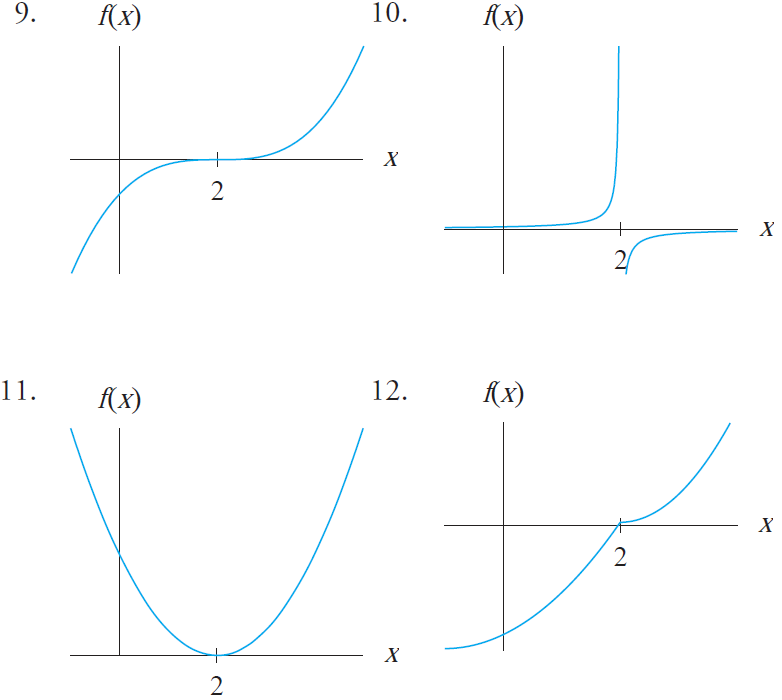
\includegraphics[scale=.8]{./img/sec42-1.png}
			\end{flushleft}
		\end{ex}
		
	\clearpage
\end{document}